\section{Exercise 2 - Implement Linear Pipeline for \texttt{MPI\_Bcast} and \texttt{MPI\_Reduce}}

The goal of exercise 2 is to implement linear pipelined versions of \texttt{MPI\_Bcast()} and \texttt{MPI\_Reduce()} 
based on the algorithms discussed in the lecture 
(Algorithms 16 and 17 in \cite{lecture_notes_traeff_collectives}). \\

\begin{figure}[h]
    \begin{center}
        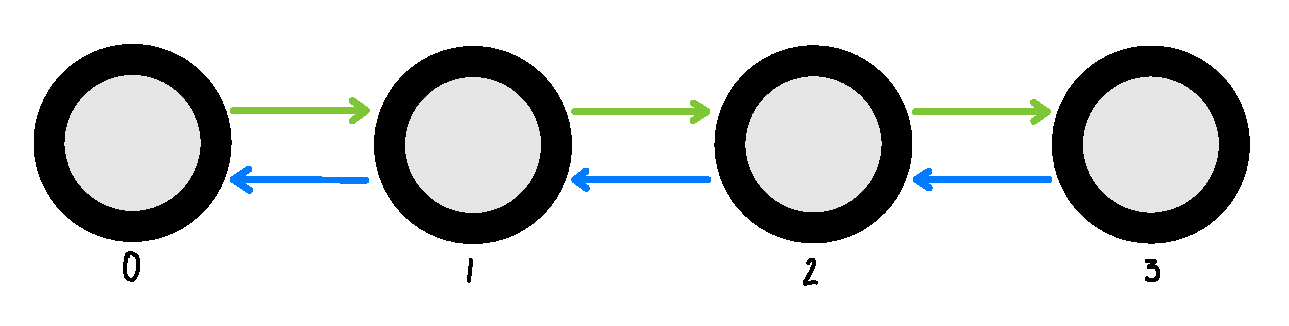
\includegraphics[width=0.7\linewidth]{figures/sketch_linear.pdf}
        \caption{Linear structure for message passing scheme in 
        exercises 2 and 3 where 0 is the root node.}
        \label{Ex2_sketch_p}
    \end{center}
\end{figure}

Our implementation for the pipelined reduction -- \texttt{MY\_Reduce\_P()} -- aligns with the following idea: We 
distinct between a master process (rank $= 0$), interior processes ($0 <$ rand $<$ size $-1$) and an end process 
(rank $=$ size $-1$). As an output of \texttt{MY\_Reduce\_P()}, the master shall possess the entry-wise maximum as 
reduction result. Additionally, we divide the array that needs to be compared into multiple blocks of size 
\texttt{blockSize} (and probably a smaller block in the end). Goal is to communicate between the processes for each 
block separately.  \\

The end process (rank $=$ size $-1$) sends blocks -- one after the other -- to the interior process with 
rank $=$ size $-2$. The end process does not receive data, as there are no further processes. Interior processes 
first receive a data block from their neighbor with rank $+1$, perform a local reduction and send this data to their 
other neighbor with rank $-1$. This is repeated for all blocks. The master process receives block data from the interior 
node of rank $=1$. \\

For performance estimation of \texttt{MY\_Reduce\_P()}, we take a look on the number of communication rounds. Let $b$ 
be the total number of blocks and $n$ the total number of processes. The number of blocks results in a latency of $b-1$ 
and for the $n$ processes are $n-1$ sucessive communications needed. In total, this leads to a maximum of $b+n-2$ 
communication rounds in \texttt{MY\_Reduce\_P()}. \\

Our implementation for the pipelined broadcast -- \texttt{MY\_Bcast\_P()} -- is quite similar to the 
\texttt{MY\_Reduce\_P()} implementation. For broadcast the goal is that the data which is I the beginning 
available for the master process shall be communicated to all the other processes. In order to do so, the master 
process sends its data block wise to its neighbor with rank $=1$ (interior process). Interior processes receive block 
data from their predecessor process and immediately communicate this data to their successor process -- block by 
block. The last one to receive the data is the end processor. There is no need to send any further data from here.\\

Very similar as for \texttt{MY\_Reduce\_P()} we can see from the implementation, that for \texttt{MY\_Bcast\_P()} 
there $b+n-2$ rounds of communication needed as well. \\

The trivial combination of \texttt{MY\_Reduce\_P()} and \texttt{MY\_Bcast\_P()} can be seen as a pipelined variant 
of \texttt{MPI\_Allreduce()}. In figure \ref{Ex2_sketch_p} the green arrows indicate communication steps for 
\texttt{MY\_Reduce\_P()} and the blue arrows \texttt{MY\_Bcast\_P()}. Once all reduction communications
are finished (green arrows), the broadcasting (blue) starts. We end up with of $2\cdot(b+n-1)$ communciation 
rounds for \texttt{MPI\_Allreduce}.

\pagebreak

\subsection*{Commutativity}

We know that \fun{MPI\_Reduce()} will start reduction from the last process and we 
also know that the function can handle non-commutative reduction operations.
In the all exercises we try to rebuild \fun{MPI\_Reduce()} and our implementation \fun{MY\_Reduce\_P()}
performs the reduction operations in the exact same order as \fun{MPI\_Reduce()}. Hence the property of handling
non-commutative operations is inherited from \fun{MPI\_Reduce()} to \fun{MY\_Reduce\_P()}.


\pagebreak
In figures \ref{Ex2_1_p} and \ref{Ex2_2_p} below, it can be observed, that the linearly pipelined algorithm outperforms
\MPIRD  $+$ \MPIBC  $ $ only for larger lenghts of count (approx. $> 5 \cdot 10^{5}$). The first one that 
outperforms it, is the one with blocksize $1 \cdot 10^4$ for both figures, meaning powers of 2 and 10. 

\begin{figure}[h]
    \begin{center}
        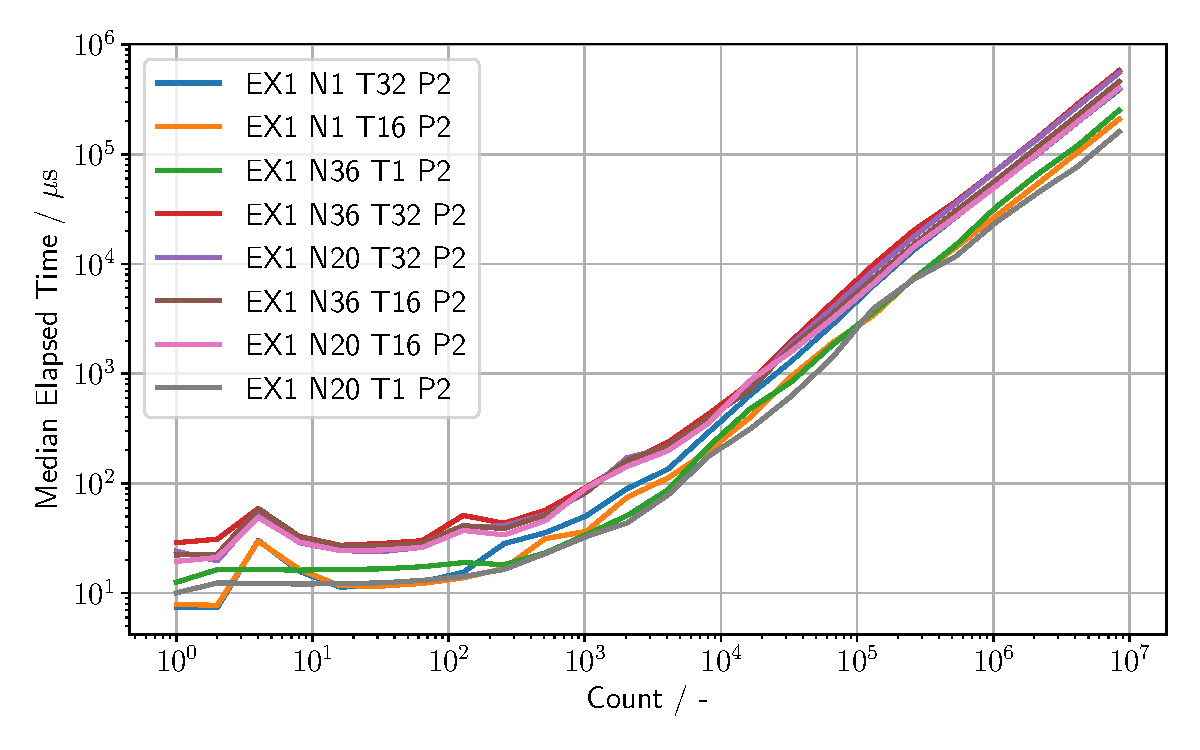
\includegraphics[width=0.7\linewidth]{figures/Ex2_1.pdf}
        \caption{Median of elapsed time for linearly pipelined reduction and broadcasting. 
        20 nodes, 16 processes per node and powers of 2.}
        \label{Ex2_1_p}
    \end{center}
\end{figure}
 
\null

\begin{figure}[h]
    \begin{center}
        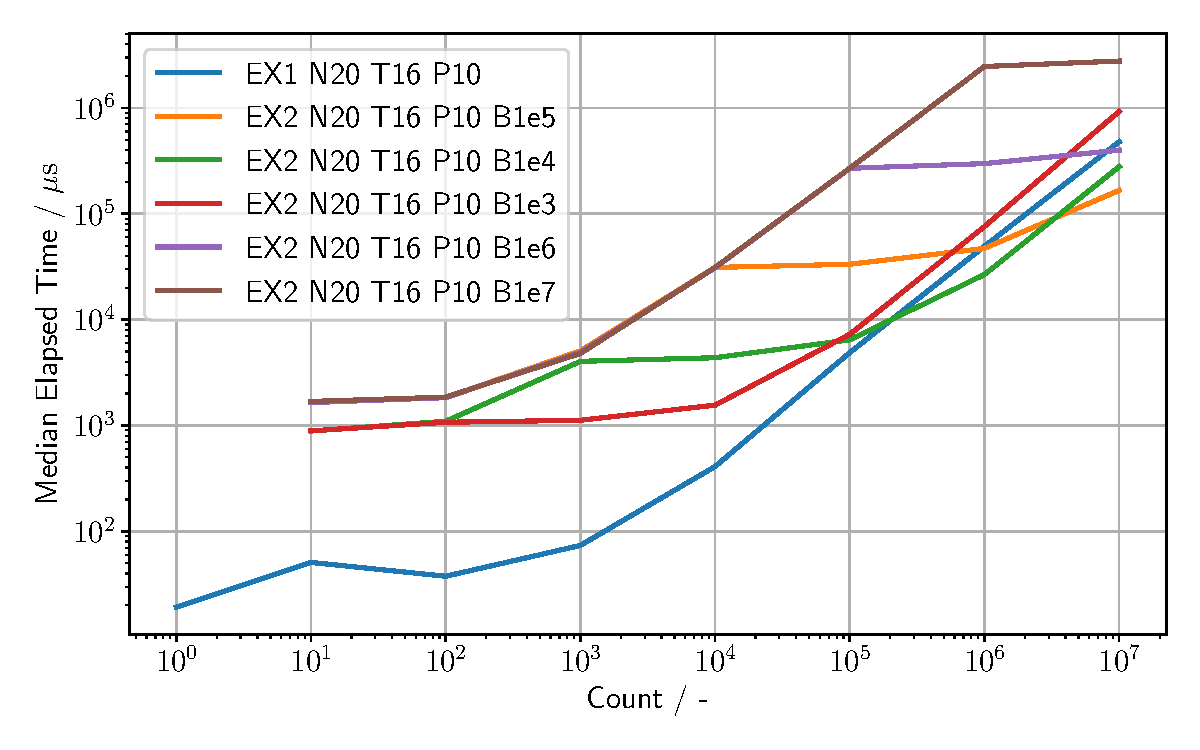
\includegraphics[width=0.7\linewidth]{figures/Ex2_2.pdf}
        \caption{Median of elapsed time for linearly pipelined reduction and broadcasting. 
        20 nodes, 16 processes per node and powers of 10.}
        \label{Ex2_2_p}
    \end{center}
\end{figure}



\pagebreak

In the following two figures \ref{Ex2_3_p} and \ref{Ex2_4_p} and \ref{Ex2_5_p} we can observe
the benefits of the different blocksizes for each configuration. For increasing
count, the execution of \fun{MY\_Reduce\_P()} and \fun{MY\_BCast\_P()}  appears to benefit from larger
blocksizes, since the slopes of the timing graphs are less steep after they reach a certain number of count.


\begin{figure}[h]
    \begin{center}
        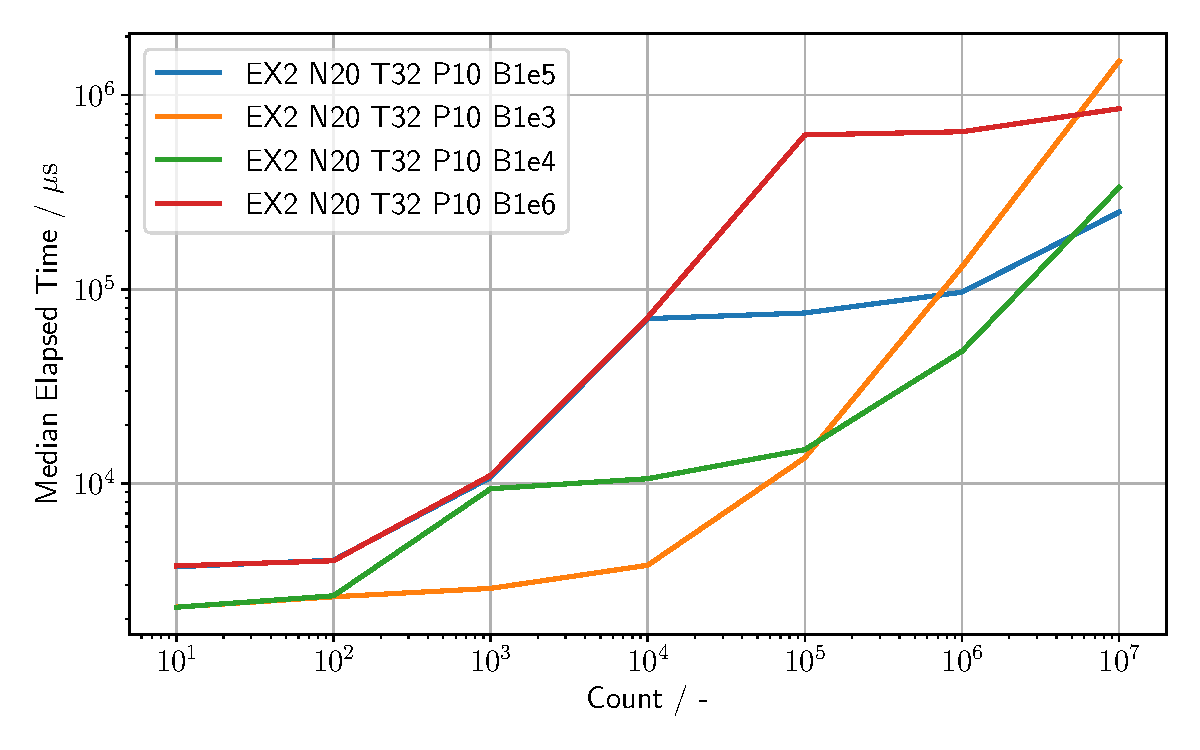
\includegraphics[width=1.0\linewidth]{figures/Ex2_3.pdf}
        \caption{Caption for Ex2 plot 3}
        \label{Ex2_3_p}
    \end{center}
\end{figure}



\begin{figure}[h]
\centering
    \begin{minipage}{.5\textwidth}
        \centering
        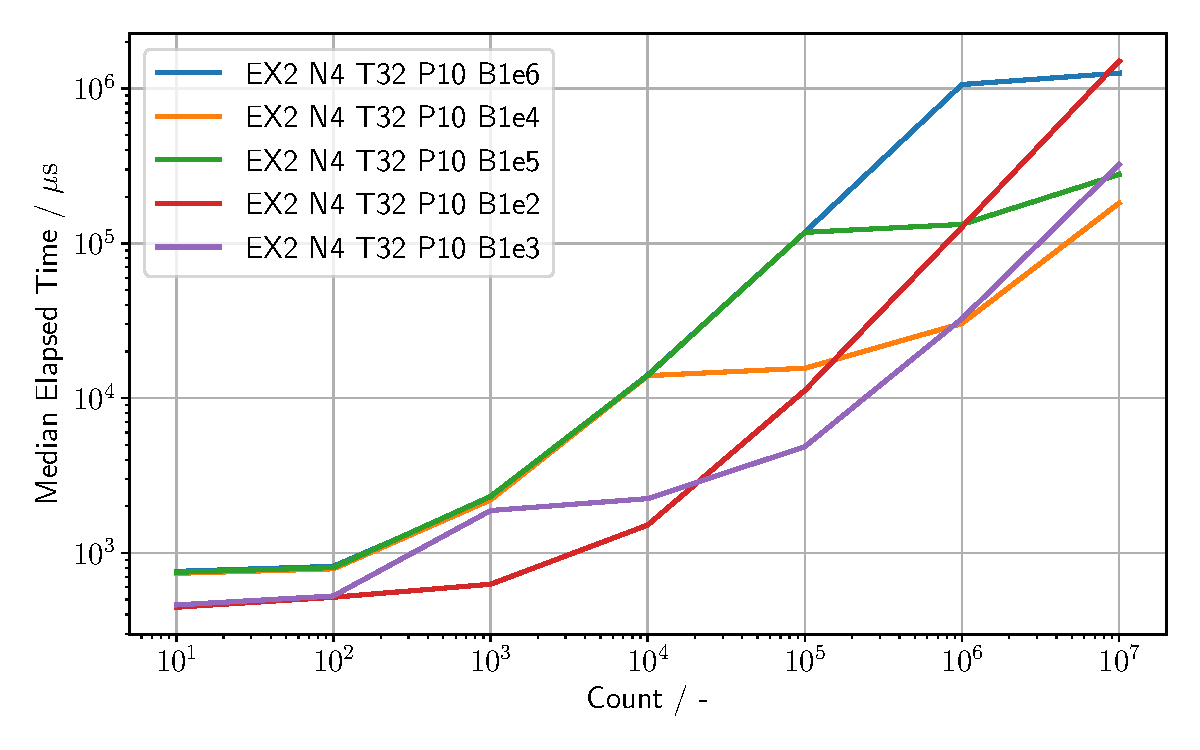
\includegraphics[width=1.0\linewidth]{figures/Ex2_4.pdf}
        \captionof{figure}{Caption for Ex2 plot 4}
        \label{Ex2_4_p}
    \end{minipage}%
    \begin{minipage}{.5\textwidth}
        \centering
        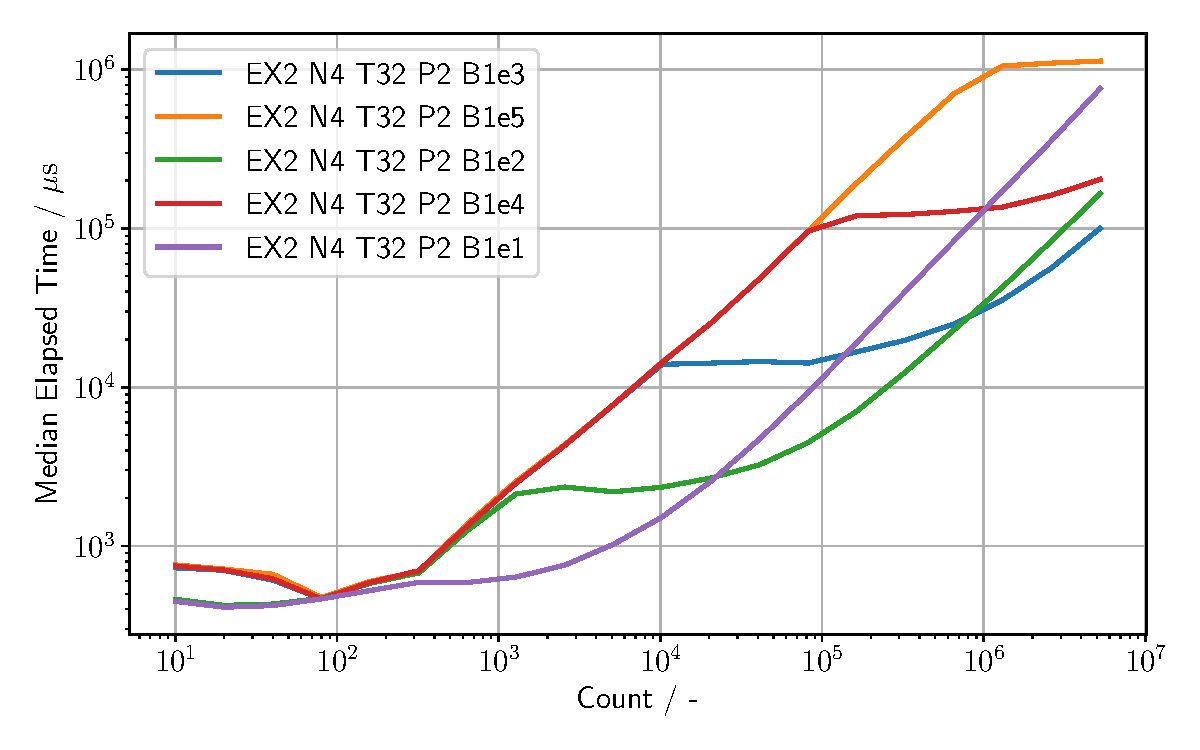
\includegraphics[width=1.0\linewidth]{figures/Ex2_5.pdf}
        \captionof{figure}{Caption for Ex2 plot 5}
        \label{Ex2_5_p}
    \end{minipage}
\end{figure}

The same pattern can be observed for both configurations (Powers of 10 and 2) with 4 processes. 
In the next exercise, we will introduce a variable blocksize that is dependent on the number count.


